\begin{frame} %=================================================================
  \frametitle{Introduction Contents}

\begin{block}{}
\begin{wideitemize}
  \item What / how / why
\end{wideitemize}
\end{block}

\end{frame} %-------------------------------------------------------------------
\note{}
%###############################################################################
%###############################################################################
%###############################################################################
%###############################################################################
\begin{frame} %=================================================================
\frametitle{What?}

\begin{center}
  \textit{Robust Decentralized Control of Cooperative Multi-robot Systems}\\[4ex]
\end{center}

\begin{block}{}
\begin{wideitemize}
  \item \textit{Simultaneous} control of \textit{multiple} systems
  \item Decentralized: \textit{no} central control authority
  \item Robust: uncertainty \textit{is} present
  \item Cooperative: an agent-binding, resource-sharing task
\end{wideitemize}
\end{block}

\end{frame} %-------------------------------------------------------------------
\note{So, what is it that I will be to you talking about? Let's break it down:

1. First of all we are interested in controlling multiple systems, that operate
in the same space, at the same time\dots

2. \dots these systems do not obey the commands of a central, shared control
authority, but decide their actions on their own \dots

3. \dots under the presence of a disturbance of some sort

4. Lastly, these systems are somehow binded in a shared activity}
%###############################################################################
%###############################################################################
%###############################################################################
%###############################################################################
\begin{frame} %=================================================================
  \frametitle{Cooperation realizations (1/2)}

\begin{figure}[H]
  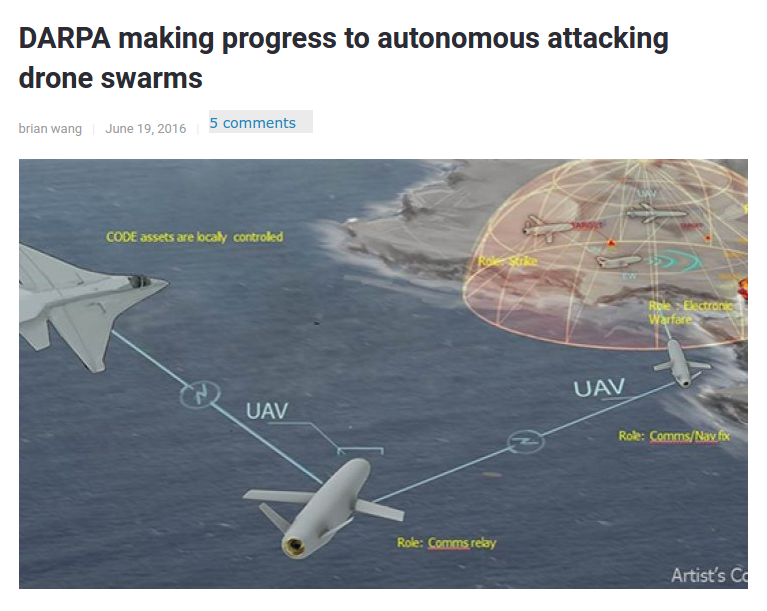
\includegraphics[scale=0.25]{figures/darpa_relay.png}
  \caption{Controller$-$Relay$-$End effector (Goals-setter $-$ autonomous agents)}
  \label{im:darpa_relay_1}
\end{figure}

Sources: \url{http://bit.ly/2pTljEf},\ \ \url{http://bit.ly/2qt1kOW}


\end{frame} %-------------------------------------------------------------------
\note{For instance, DARPA is interested in controlling swarms of drones whose
  members may need to act as relays of information, due to the fact that
  communication ranges are not limitless.}
%###############################################################################
%###############################################################################
%###############################################################################
%###############################################################################
\begin{frame} %=================================================================
  \frametitle{Cooperation realizations (2/2)}

\begin{minipage}{0.45\textwidth}
\begin{figure}[H]
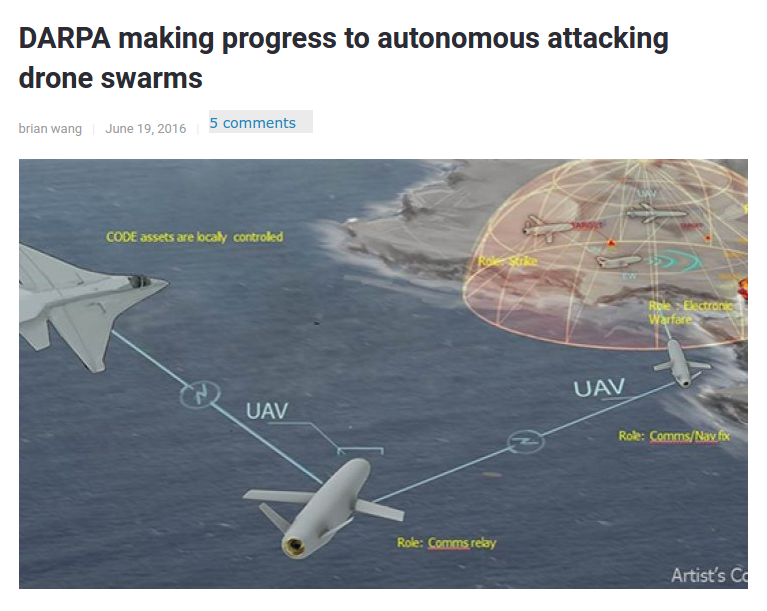
\includegraphics[scale=0.25]{figures/darpa_relay.png}
  \caption{Controller$-$Relay$-$End effector (Goals-setter $-$ autonomous agents)}
  \label{im:darpa_relay_2}
\end{figure}
\end{minipage} \hfill
\begin{minipage}{0.4\textwidth}
Prerequisites-tier:
\begin{itemize}
\item Connectivity maintenance
\item Collision avoidance (agents plus obstacles)
\end{itemize}
\end{minipage}

\end{frame} %-------------------------------------------------------------------
\note{In any case, we find that there are two fundamental prerequisites of
  cooperation in decentralized settings: an arbitrary agent needs to maintain
  connectivity with a set of agents, and avoid colliding with them, and any
  obstacle that it may come across.

  In this context, there are two interesting areas of control:}
%###############################################################################
%###############################################################################
%###############################################################################
%###############################################################################
\begin{frame} %=================================================================
  \frametitle{Control in what sense? (1/2)}

  Reference tracking

\begin{figure}[H]\centering
  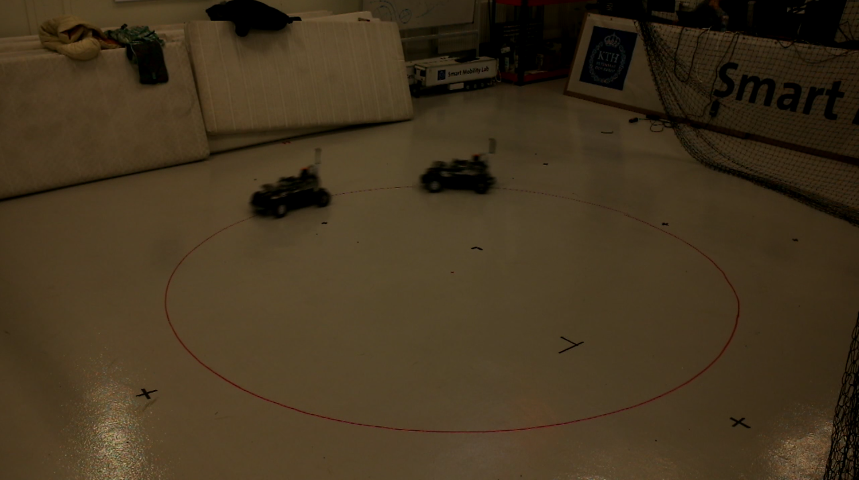
\includegraphics[scale=0.3]{figures/tcars.png}
  \caption{Vehicles tracking a desired trajectory in tandem.}
  \label{im:tracking_mention}
\end{figure}

\end{frame} %-------------------------------------------------------------------
\note{  The first is trajectory tracking, where either an agent all the whole
  multi-agent system needs to follow a given trajectory as close as possible,
  and stabilization\dots}
%###############################################################################
%###############################################################################
%###############################################################################
%###############################################################################
\begin{frame} %=================================================================
  \frametitle{Control in what sense? (2/2)}

  Stabilization\\[2ex]

\begin{minipage}{0.45\textwidth}
\begin{tikzpicture}[remember picture]
   %\node[anchor=south west, inner sep=0pt] at (current page.south west) {%
   \node[anchor=south west, inner sep=0pt] at (1.5,-3) {%
     \movie[height = 0.5\paperheight, width = 0.72\paperwidth, poster, showcontrols, autostart,loop] {}{figures/tank_stable.mp4}%
   };
\end{tikzpicture}
\end{minipage}

source: \url{http://www.popularmechanics.com/military/weapons/a18362/tank-carry-beer/}

\end{frame} %-------------------------------------------------------------------
\note{where for instance each agent is assigned a desired configuration to which
  he must arrive at some point and stay, regardless of disturbances affecting
  his dynamic behaviour. I found this video of stabilization on the internet
  to be quite impressive.

  And this is what the goal of this thesis is: to stabilize a multi-agent
  system subject to disturbances to predefined configurations for all
  agents. More or less we are interested in achieving this:}
%###############################################################################
%###############################################################################
%###############################################################################
%###############################################################################
\begin{frame} %=================================================================
\frametitle{In particular: stabilization}
\begin{tikzpicture}[remember picture,overlay]
   %\node[anchor=south west, inner sep=0pt] at (current page.south west) {%
   \node[anchor=south west, inner sep=0pt] at (1.5,-3) {%
     \movie[height = 0.5\paperheight, width = 0.72\paperwidth, poster, showcontrols, autostart,loop] {}{figures/trajectories_only_loss.avi}%
     %\movie[height = 0.5\paperheight, width = 0.72\paperwidth, poster, showcontrols, loop] {}{figures/trajectories_only_lossless.avi}%
   };
\end{tikzpicture}

\end{frame} %-------------------------------------------------------------------
\note{What we see here are three agents that have to somehow bypass two obstacles

1. without the blue agent losing connectivity with the other two, and
2. without all of them crashing into agents or obstacles

prior to stabilizing themselves in some chosen configuration.}
%###############################################################################
%###############################################################################
%###############################################################################
%###############################################################################
\begin{frame} %=================================================================
\frametitle{How?}

  \begin{center}
    \textit{an inter-constraint Receding Horizon approach}\\[4ex]
  \end{center}

  \begin{block}{}
  \begin{wideitemize}
    \item ordinary Receding Horizon / Model Predictive Control strategy
    \item cooperating agents are \textit{inter-constrained}
  \end{wideitemize}
  \end{block}

\end{frame} %-------------------------------------------------------------------
\note{Now, how did we achieve this?

We used the control strategy of Receding Horizon (or Model Predictive) Control,
where the connectivity and collision avoidance mandates are incorporated
as constraints}
%###############################################################################
%###############################################################################
%###############################################################################
%###############################################################################
\begin{frame} %=================================================================
  \frametitle{Why MPC?}

  \begin{wideitemize}
    \item direct incorporation of connectivity / collision constraints
    \item direct incorporation of input / state constraints
    \item theoretic guarantees of stability
    \item effective in aspects other methods are not
  \end{wideitemize}

\end{frame} %-------------------------------------------------------------------
\note{Why choose MPC over any other strategy?

  MPC has the unique advantage that it can directly incorporate

  1. the type of constraints we are interested in imposing
  2. input / state constraints

  a. we can procure theoretic guarantees of stability
  b. it can be effective in aspects other methods are not}
%###############################################################################
%###############################################################################
%###############################################################################
%###############################################################################
\begin{frame} %=================================================================
  \frametitle{Prior approaches}

  \begin{wideitemize}
    \item Navigation Functions
    \item Cost-coupled Decentralized MPC
  \end{wideitemize}

\end{frame} %-------------------------------------------------------------------
\note{For instance the same problem was approached using navigation functions,
  but this way proved to be not as robust as MPC.

  The superiority of MPC has been exploited previously, and some approaches
  consider imposing the kinds of constraints we are interested in by
  coupling systems through the cost functions that MPC uses, instead of
  through their constraints.}
